%HEADER

%<---!!!!!!!!!!!!!!! MAKRO-DEFIONITIONEN; BITTE NICHT VERAENDERN !!!!!!!!!!
%<--- ARBEIT EINSEITIG
\def\makroEinseitig{
%KOMA-Script-Klasse: scrreprt
%deutsches Design, Schriftgröße 12, DIN A4
%Literaturverzeichnis und Index in Inhaltsverzerzeichnis einbinden
\documentclass[12pt,a4paper,listof=totoc,oneside]{scrreprt}
%Seitenspiegel einstellen
\usepackage[a4paper]{geometry}
\geometry{a4paper,left=30mm,right=25mm,
bottom=20mm,top=15mm,bindingoffset=2mm,
includehead,includefoot}}
% ARBEIT EINSEITIG --->

\def\makroZweiseitig{
%<--- ARBEIT ZWEISEITIG
%KOMA-Script-Klasse: scrreprt
%deutsches Design, zweiseitig
%Literaturverzeichnis und Index in Inhaltsverzerzeichnis einbinden
\documentclass[12pt,a4paper,listof=totoc,twoside, headsepline]{scrreprt}
\usepackage[a4paper]{geometry}
\geometry{a4paper,left=25mm,right=25mm,
bottom=20mm,top=15mm,bindingoffset=2mm,
includehead,includefoot}}
% ARBEIT ZWEISEITIG --->

%<--- Einstellungen Kopfzeile
\def\makroFH-Kopfzeilenstil{
\pagestyle{scrheadings} 
\setheadsepline{0.4pt}
\pagestyle{scrheadings}
\renewcommand*{\chapterpagestyle}{scrheadings}}
%Einstellungen Kopfzeile --->
%!!!!!!!!!!!!!!! MAKRO-DEFIONITIONEN; BITTE NICHT VERAENDERN !!!!!!!!!!--->


%AUSWAHL: TEXT EINSEITIG (ja/nein)
\makroEinseitig
%\makroZweiseitig

%schalte Umlaute frei
\usepackage[english, ngerman]{babel}
%passende Codierung
\usepackage[utf8]{inputenc}
%Seitenspiegel einzustellen
\usepackage[a4paper]{geometry}

%%%%%%%%%%%%%%%%%%%%%%%%%%%%%%%%%%%%%%%%%%%%%%%%%%%%%%%%%%%%%%%%%%%%%%%%%%%%%%%%
% Deutsche und englische Referenzen
\usepackage{babelbib}

% Utopia Schriftart
\usepackage{utopia}

% Farbige Überschriften
% https://www.overleaf.com/learn/latex/Using_colours_in_LaTeX
\usepackage[dvipsnames]{xcolor}
\usepackage{sectsty}
\chapterfont{\color{CornflowerBlue}}
\sectionfont{\color{Cerulean}}
\subsectionfont{\color{Cerulean}}
\subsubsectionfont{\color{Cerulean}}
\paragraphfont{\color{Cerulean}}
%%%%%%%%%%%%%%%%%%%%%%%%%%%%%%%%%%%%%%%%%%%%%%%%%%%%%%%%%%%%%%%%%%%%%%%%%%%%%%%%

%Mathepaket
\usepackage{amsmath}
%Symbole
\usepackage{amssymb}
%griechische Symbole
\usepackage{upgreek}
%weitere Symbole
\usepackage{pxfonts}
% Phonetischen Alphabete für LaTeX
\usepackage{tipa}
%farbige Schriften
%\usepackage{color}
\usepackage{scrhack}
%Bilder fixieren
\usepackage{float}
%Grafiken einbinden
\usepackage{graphicx}
% Kopf- und Fußzeilen
\usepackage[automark,standardstyle,markusedcase]{scrlayer-scrpage}
% deutsche Überschriften
\usepackage[ngerman]{translator}
% Kopfzeilenabstand festlegen
\setlength{\headheight}{10mm}
%Abb. statt Abbildung
\usepackage{caption3}
\addto\captionsngerman{
\renewcommand{\figurename}{Abb.}
\renewcommand{\tablename}{Tab.}
}
%Glossar-Pakage
% HYPERREF VOR GLOSSARIES EINFÜGEN
\usepackage{hyperref}

\usepackage[
nonumberlist, %keine Seitenzahlen anzeigen
acronym,      %ein Abkürzungsverzeichnis erstellen
toc]          %Einträge im Inhaltsverzeichnis      
{glossaries}
\usepackage{cite}

\hypersetup{ colorlinks,
linkcolor=MidnightBlue,
filecolor=MidnightBlue,
urlcolor=MidnightBlue,
citecolor=MidnightBlue }

%Glossar einschalten
\makeglossaries


%fertigen Kopfzeilenstil aktivieren
\makroFH-Kopfzeilenstil

%Zeilenabstand * 1.25 (default)
\renewcommand{\baselinestretch}{1.25}\normalsize
%(Kommentar entfernen, um Zeilenabstand
% auf 1,5-fache Groesse zu ueberschreiben)
%\renewcommand{\baselinestretch}{1.50}\normalsize

% KOMPILATION
% pdflatex Arbeit_Main.tex
% makeglossaries Arbeit_Main
% bibtex Arbeit_Main
% 2 * pdflatex Arbeit_Main.tex
%

% https://www.overleaf.com/learn/latex/Tables
\setlength{\arrayrulewidth}{0.5mm}
\setlength{\tabcolsep}{18pt}
\renewcommand{\arraystretch}{1.5}

\newcommand{\todo}[1]{\textcolor{red}{\textbf{TODO #1}}}
\newcommand{\xcom}{\textcolor{YellowGreen}{\textbf{[?] }}}
\newcommand{\misobj}[1]{\textcolor{YellowGreen}{\textbf{#1}}}

\begin{document}

%Befehle für Symbole
%\newglossaryentry{symb:Pi}{
%name=$\pi$,
%description={Die Kreiszahl.},
%}
%\newglossaryentry{symb:Phi}{
%name=$\varphi$,
%description={Ein beliebiger Winkel.}
%}
%\newglossaryentry{symb:Lambda}{
%name=$\lambda$,
%description={Eine beliebige Zahl, mit der der nachfolgende Ausdruck
%multipliziert wird.}
%}

%Akronyme

%\newacronym{MS}{MS}{Microsoft}

%Eine Akronym mit Glossareintrag
\newacronym{PCA}{PCA}{Primary Component Analysis\protect\glsadd{glos:PCA}}

%Glossareinträge

%\newglossaryentry{glos:AD}{
%name=Active Directory,
%description={Active Directory ist in einem Windows 2000/" "Windows
%Server 2003-Netzwerk der Verzeichnisdienst, der die zentrale ...
%}
%}

\newglossaryentry
{glos:Predictive_Analytics}{name=Predictive Analytics, description=
{Die Analyse von Daten mit Hilfe mathematischer und statistischer Methoden.
Das Ziel von Predictive Analytics ist die Erstellung von Prognosen zur
Unterstützung der Entscheidungsfindung}
}

\newglossaryentry
{glos:PCA}{name=Primary Component Analysis, description=
{Eine Methode zur Variablenreduktion. Dabei wird ein neuer Satz von
Basisvektoren berechnet, der die Varianz der Daten am Besten beschreibt}
}


%Titelseite
% Seitennummer aus
\thispagestyle{empty}
\begin{titlepage}
	\vspace{3cm}

%%\begin{center}
%%	\Huge	
%%	HOCHSCHULE LANDSHUT \\
%%	\Large
%%	FAKULTÄT INFORMATIK
%%\end{center}

%%\vspace{1cm}

\begin{center}
	
\includegraphics[scale=0.8]{Grafiken/hl-logo.pdf}  
\end{center}

\vspace{2.5cm}

\begin{center}
  \Large FAKULTÄT INFORMATIK
\end{center}

\vspace{1cm}
\begin{center}
	\Huge
	\textbf{Masterarbeit}\\
\end{center}

\vspace{1cm}

\begin{center}
	\Large
	\textsc{Predictive Analytics im öffentlichen Sektor - Anwendungsmöglichkeiten,
    Chancen und Risiken}\\
\end{center}

\vspace{1.5cm}

\begin{center}
	\Large
	Dmitrij Novikov
\end{center}

\vspace{2cm}
\begin{center}


	\large
	%\the\month\,/\,\the\year
Eingereicht am \today
\end{center}

\vspace{2cm}
\begin{center}
	\large
	Betreuer: Prof. Dr. Wunderlich
\end{center}

\end{titlepage}


%Füge leere Seite ein (optional)
\clearpage 
\ifodd\count0\else 
\thispagestyle{empty} 
\hbox{}\newpage 
\fi 
%Verwende Muster-Erklärung zur selbstständigen Arbeit 
%Erklärung
\thispagestyle{empty}
\vspace{15mm}
\begin{center}
\textbf{\underline{ERKLÄRUNG ZUR MASTERARBEIT}}
\end{center}
\vspace{25mm}
\begin{center}
\large
%Name, Vorname des Studierenden:  \\
\large
Novikov, Dmitrij
\end{center}
\vspace{25mm}

\begin{center}
\huge
Hochschule Landshut \\
Fakultät Informatik 
\end{center}
\vspace{10mm}

\begin{center}
\large
Hiermit erkläre ich, dass ich die Arbeit selbständig 
verfasst, noch nicht anderweitig für Prüfungszwecke 
vorgelegt, keine anderen als die angegebenen Quellen 
oder Hilfsmittel benützt, sowie wörtliche und sinngemäße 
Zitate als solche gekennzeichnet habe.  \\
\end{center}
\vspace{55mm}

\begin{center}
....................\hspace{40mm}....................................................\\

(Datum)\hspace{47mm}(Unterschrift des Studierenden)
\end{center}

%Füge leere Seite ein (optional)
\clearpage 
\ifodd\count0\else 
\thispagestyle{empty} 
\hbox{}\newpage 
\fi 

\begin{abstract}
\begin{center}
\Huge
\emph{\textbf{Abstract}}
\end{center}
\normalsize
\vspace{15mm}
\textit{\todo{Abstract}}
\end{abstract}


\tableofcontents
\setcounter{page}{1}

\chapter{Einleitung}
\label{part:Einleitung}

In dieser Arbeit soll die Anwendung von Datenanalysen und insbesondere
von \emph{\gls{glos:Predictive_Analytics}} im öffentlichen Sektor untersucht
werden.
Der Schwerpunkt liegt dabei auf Deutschland, wobei aber auch relevante
Anwendungsgebiete in anderen Staaten betrachtet werden. \\ \\
Der einleitende Teil~\ref{part:Schw_Vorhersagen} soll zunächst das Problem der
Schwierigkeit von
Prognosen untersuchen und damit eine Motivation für die Anwendung von 
\emph{predictive analytics} liefern. \\ \\
In Teil~\ref{part:Konzepte_PA} werden die wichtigsten Konzepte von
\emph{predictive analytics} vorgestellt. Dabei werden auch die allgemeinen
Risiken bei der Anwendung diskutiert. \\ \\
\misobj{weitere Teile}

\chapter{Die Schwierigkeit von Vorhersagen}
\label{part:Schw_Vorhersagen}

Mit Hilfe von \emph{\gls{glos:Predictive_Analytics}} werden Datenanalysen
erstellt, die die Vorhersage von Entwicklungen oder die Einschätzung von
Situationen unterstützen sollen. Dabei werden in der Regel Computeralgorithmen
mit Daten trainiert, um für spätere Abfragen zuverlässige Prognosen zu liefern.
Entscheidungsträgern soll \emph{predictive analytics} also helfen, bessere
strategische Entscheidungen zu treffen (vgl. \cite{Mauerer}, S.~2). %\\ \\
Dies könnte
\begin{description}
\item[(a)] notwendiger sein als erwartet und
\item[(b)] schwieriger werden als gedacht.
\end{description}
Denn eine ausführliche Studie des Psychologen Philip Tetlock aus dem Jahr 2005
(siehe \cite{Tetlock}) ergab,
dass Experten zu politischen Fragen keine besseren Prognosen liefern konnten,
als die einfachsten statistischen Algorithmen. Zudem hatten die Experten
große Schwierigkeiten damit, ihre Prognosen angesichts schlechter Resultate
anzupassen und zu verbessern. \\ \\
Die Experten sollten ihr Können bei mehreren Prognoseaufgaben
(\emph{forecasting exercises}) unter Beweis stellen. Dabei wurden verschiedene
mögliche politische oder wirtschaftliche Ereignisse skizziert und die Experten
sollten subjektiv abschätzen, für wie wahrscheinlich sie es halten, dass das
Ereignis eintritt\footnote{Es sollten numerische Werte angegeben werden. Also
0 für \glqq{Es} ist unmöglich, dass das Ereignis eintritt\grqq und 1 für
\glqq{Das} Ereignis wird mit Sicherheit eintreten\grqq. Werte zwischen 0 und 1
drücken dann einen Grad von Unsicherheit über das Ereignis aus.}.
Nachdem das festgelegte Zeitfenster für die Ereignisse abgelaufen war, konnte
das Eintreten oder Nichteintreten der jeweiligen Szenarien beobachtet werden und
rückblickend mit den Vorhersagen der Teilnehmer abgeglichen werden.  
Zur Messung der Genauigkeit der Vorhersagen wurde eine Maßzahl,
der \emph{probability score} verwendet. Dabei wurden ihre Vorhersagen mit den
Ergebnissen von einfachen und erweiterten statistischen Algorithmen
verglichen. \\ \\
Das Ergebnis ist in Abbildung~\ref{pic:Tetlock_1} dargestellt und wird im
folgenden Text ausführlich erläutert\footnote{Die Grafik ist eine leicht 
abgewandelte Version vom Original aus \cite{Tetlock}, S. 51).}. \\ \\
\begin{figure}%[!hbt]
\centering
\caption{Bei den \emph{forecasting exercises} erzielte Wertungen.}
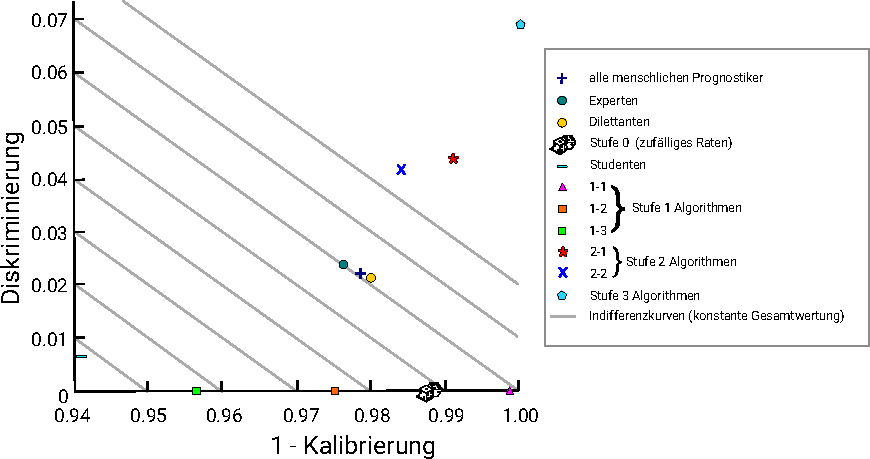
\includegraphics[scale=1.0]{Grafiken/Tetlock_1_Fertig_Ink.pdf} 
\label{pic:Tetlock_1}
\end{figure}
Die zwei
Bestandteile des \emph{probability score}, Kalibrierung (\emph{calibration}) und
Diskriminierung (\emph{discrimination}), sind auf den Achsen abgebildet. \\ \\ 
Kalibrierung (horizontale Achse) misst die Fähigkeit eines Prognostikers,
Ereignisse korrekt nach ihrer
Auftrittswahrscheinlichkeit zu ordnen (vgl. \cite{Tetlock}, S.~47). So ist ein
Prognostiker gut kalibriert, wenn etwa 10~\% der Ereignisse eintreten, für die
er eine Wahrscheinlichkeit von 0.1 geschätzt hat, 20~\% der Ereignisse eintreten
die eine Wahrscheinlichkeit von 0.2 erhalten haben, und so weiter. Je kleiner
der numerische Wert der Kalibrierung, desto besser ist der Prognostiker. Bei
einem Wert von 0 ist die bestmögliche Kalibrierung erreicht und aus diesem Grund
ist (1 - Kalibrierung) auf der horizontalen Achse abgebildet. \\ \\
Weiterhin ist ein Prognostiker umso besser bei der Diskriminierungskomponente
(vertikale Achse),
je eher es ihm gelingt die Auftrittswahrscheinlichkeiten von einzelnen
Ereignissen von der relativen Häufigkeit aller Ereignisse\footnote{
genauer: Das Verhältnis der Anzahl der eingetretenen Ereignisse zu der
Gesamtanzahl der Ereignisse} (\emph{base-rate})
zu unterscheiden. Perfekte Diskriminierung wird erreicht, wenn allen 
eingetretenen Ereignissen eine Wahrscheinlichkeit von 1.0 zugeordnet wird, und
alle Ereignisse, die nicht eingetreten sind, mit Null bewertet werden
(vgl. \cite{Tetlock}, S.~47).\\ \\
Nun gehen Kalibrierung und Diskriminierung als Summe in den
\emph{probability score} ein. Aus diesem Grund kann sich für verschiedene
Werte von Kalibrierung und Diskriminierung der gleiche Wert für den
\emph{probability score} ergeben. Die diagonalen Linien in Abbildung~\xcom
markieren Stellen mit konstantem \emph{probability score}. Je weiter rechts oben
eine Linie verläuft, desto höher ist der zugehörige \emph{probability score}.
\\ \\
Die Gesamtergebnisse für Kalibrierung und Diskriminierung für die verschiedenen
Teilnehmergruppen sind in der Graphik eingetragen. Die am besten qualifizierte
Gruppe stellen die Experten dar, die Fragen zu ihren jeweiligen Fachgebieten
erhalten haben (vgl. \cite{Tetlock}, S.~242). Weniger qualifiziert sind die 
\glqq{Dilettanten}\grqq (\emph{dilettantes}), Experten, die jedoch Fragen
beantwortet haben, die nicht zu ihrem Spezialgebiet gehören. Die Dilettanten
gaben an, dass sie sich mit Hilfe qualititativ hochwertiger Quellen
(\emph{Economist}, \emph{Wall Street Journal}, \emph{New York Times} etc.) über
Themen außerhalb ihrer Fachgebiete informieren (vgl. \cite{Tetlock}, S.~56).
Die Gruppe mit der geringsten Qualifikation waren Studenten, die die Übungen
zu Vorhersagen absolvieren mussten, nachdem sie kurze Zusammenfassungen von
Fakten zu den jeweiligen Themen erhalten haben (vgl. \cite{Tetlock}, S.~56).
\\ \\
Weiterhin enthält Abbildung~\ref{pic:Tetlock_1} auch die Ergebnisse, die von den
statistischen Algorithmen erzielt wurden. Zur besseren Übersicht werden die
Algorithmen hier in vier Gruppen eingeteilt. Der Stufe 0 Algorithmus würfelt
einfach die Antworten , er ordnet den zur Debatte stehenden Ereignissen
zufällige Wahrscheinlichkeiten zu. Weiterhin gibt es mehrere Varianten von
Stufe 1 Algorithmen, die als Antwort auf die Fragen immer die relative
Häufigkeit der Ereignisse eintragen. Etwas komplexer sind die Stufe 2
Algorithmen. Diese extrapolieren aus der Vergangenheit in die Zukunft und setzen
die Wahrscheinlichkeiten für die Ereignisse entsprechend. Die höchste
Komplexität hat der Stufe 3 Algorithmus. Um die Eintrittswahrscheinlichkeiten
der Ereignisse zu ermitteln, nutzt dieser die Vergangenheitswerte mehrerer
Variablen, die eine hohe Vorhersagekraft besitzen.\footnote{Die genaue Zuordnung
der Stufen 0-3 zu den Algorithmen in der Originalquelle (\cite{Tetlock}, S.~51)
sieht folgendermaßen aus:
\begin{description}
\item[Stufe 0:] \emph{random guessing} (\emph{chimp})
\item[Stufe 1:] \emph{contemporary base rate} (1-1), \emph{restrictive base
  rate} (1-2), \emph{expansive base rate} (1-3)
\item[Stufe 2:] \emph{cautious case-specific extrapolation} (2-1),
  \emph{aggressive case-specific extrapolation} (2-2)
\item[Stufe 3:] \emph{autoregressive distributed lag models}
\end{description}
} \\ \\
Abbildung~\ref{pic:Tetlock_1} zeigt, dass die Experten die Studenten bei
den \emph{forecasting exercises} deutlich schlagen konnten. Allerdings waren die
Experten kaum besser (!) als der zufallsgesteuerte Algorithmus 
(Stufe 0)\footnote{Die Experten waren schlechter kalibriert aber besser bei
der Diskriminierung, sodass sie insgesamt eine etwas bessere Gesamtwertung
hatten}. Insbesondere verloren die Experten gegen die komplexeren Algorithmen
(Stufe 2 und 3) mit deutlichem Abstand und zwar sowohl bei Kalibrierung, als
auch bei Diskriminierung. Falsche Überzeugungen und mentale Barrieren haben, so
Tetlock, das Urteilsvermögen der Experten getrübt und zu den schlechten
Ergebnissen geführt (mehr dazu in Abschnitt~\xcom). \\ \\
Was haben diese Ergebnisse mit \emph{predictive analytics} und dem öffentlichen
Sektor zu tun?\\ \\
Erstens waren die Fragestellungen der \emph{forecasting exercises} aus den
Bereichen Politik und Wirtschaft\footnote{
Andere Themen, wie beispielweise naturwissenschaftliche Fragestellungen,
z. B. \glqq{Wie} wahrscheinlich ist die Detektion dunkler Materie
in den nächsten fünf Jahren?\grqq, wurden nicht behandelt.
}, was für den öffentlichen Sektor relevant ist. Zweitens handelt es sich dabei
um generelle Probleme der menschlichen Urteilsfindung. Probleme, die in vielen
Bereichen auftreten und zu Fehleinschätzungen führen können. Zudem
konnten datenbasierte Algorithmen, also \emph{predictive analytics}, die
menschlichen Vorhersagen bei den \emph{forecasting exercises} schlagen. Dies
deutet darauf hin, dass formale Methoden wie \emph{predictive analytics} dabei
helfen können, bessere Urteile zu fällen und folglich auch bessere
Entscheidungen zu treffen. \\ \\
Der nächste Teil der Arbeit behandelt \emph{predictive analytics},
den Prozess der (menschlichen) Urteilsfindung und wie formale Methoden diesen
Prozess verbessern können.


\chapter{Konzepte von Predictive Analytics}
\label{part:Konzepte_PA}

\section{Begriffsdefinition und -Abgrenzung}

Das primäre Ziel von \emph{\gls{glos:Predictive_Analytics}} ist das Treffen von
Vorhersagen.
Hierbei sind nicht nur Prognosen für die Zukunft gemeint, sondern
auch Einschätzungen und Beurteilungen unklarer Situationen, bei denen die für
die Entscheidungsfindung wichtigen Daten fehlen (vgl. \cite{Dinov}, S.~9~f.).
Hier sind einige Anwendungsbeispiele, die verdeutlichen, wie \emph{predictive
analytics} eingesetzt werden kann (vgl. \cite{Schmitz}):
\begin{description}
\item[Betrugserkennung (\emph{fraud detection}):] Geschäftsvorgänge werden
automatisch analysiert, in der Hoffnung, dass Unregelmäßigkeiten vom System
erkannt werden. Verdächtige Vorgänge können dann zum Beispiel einer manuellen
Prüfung unterzogen werden.
\item[Vorhersage von Wartungszeitpunkten (\emph{predictive maintenance}):]
Automatische Systeme schätzen die Ausfallwahrscheinlichkeit von Maschinen ein
und bestimmen den Zeitpunkt für die nächste Inspektion.
\item[Verringerung von Ausschuss (\emph{predictive quality}):]
Mit Hilfe von Sensordaten werden fehlerhafte Produkte im Produktionsprozess
erkannt und aussortiert.
\item[Erkennung von Kundenunzufriedenheit (\emph{churn management}):]
Muster in Daten, die auf Unzufriedenheit von Kunden deuten, automatisch erkennen
und rechtzeitig Gegenmaßnahmen versuchen.
\item[Verbesserung der Zahlungsmoral:]
Mit Hilfe von Vorhersagen die Randbedingungen verbessern, sodass Kunden
schneller Rechnungen begleichen.
\item[Bessere Kontrolle von Personalfluktuationen:]
Mitarbeiter, die bald einen Arbeitsplatzwechsel vollziehen könnten, mit Hilfe
von Vorhersagemodellen erkennen, um rechtzeitig darauf reagieren zu können.
\end{description}
\begin{figure}%[!hbt]
\centering
\caption{Erstellung von Vorhersagemodellen.}
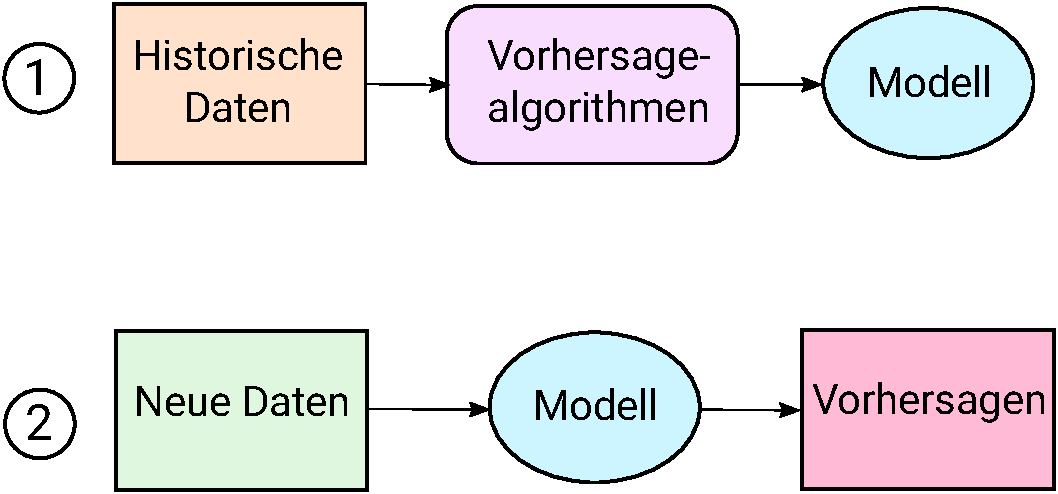
\includegraphics[scale=0.8]{Grafiken/PA_Ink.pdf} 
\label{pic:PA}
\end{figure}
Abbildung~\ref{pic:PA} veranschaulicht den allgemeinen Prozess zur Generierung
von Vorhersagemodellen\footnote{
Basierend auf dem Original aus \cite{Parthasarathy}.
}.
Zum Erstellen der Vorhersagen werden historische Daten benötigt. Diese Daten
werden von Algorithmen genutzt, um Modelle zu bauen. Die Vorhesagemodelle
akzeptieren neue Daten als Eingabe und liefern dazu eine Vorhesage der
gewünschten Eigenschaften. So könnte eine Versicherung beispielsweise
Vorhersagemodelle zur Betrugserkennung implementieren. Die historischen Daten
könnten in diesem Fall Forderungen von Kunden an die Versicherung aus der
Vergangenheit sein. Das Vorhesagemodell würde dann eine neue Forderung an die
Versicherung als Eingabe nehmen und könnte als Ausgabe eine Zahl zwischen 0 und
1 liefern. Dieser vorhergesagte Wert kann dann als Wahrscheinlichkeit
interpretiert werden, dass es sich bei der neuen Forderung um einen Betrugsfall
handelt. 


\section{Probleme menschlicher Urteile}

Die meisten Urteile und Prognosen werden von Menschen gefällt, ohne statistische
Modelle und Vorhersagealgorithmen zu nutzen. Grundsätzlich fällt jeder Mensch
Urteile, macht Vorhersagen und nutzt diese um Entscheidungen zu treffen. Aus
diesem Grund ist ein gutes Urteilsvermögen eine Eigenschaft, die eigentlich
universell gebraucht wird. Für die großen gesellschaftlichen Entscheidungen
versorgen Experten Wirtschaft, Politik und Öffentlichkeit mit Prognosen und
Einschätzungen. Dabei ist es üblich routinemäßig Expertenmeinungen einzuholen,
unüblich ist es allerdings, systematisch die Qualität dieser Urteile zu
überprüfen (vgl. \cite{Tetlock}, S.~1). Aus diesem Grund hat der Psychologe
Philip Tetlock sich zur Aufgabe gemacht, \glqq{gutes} Urteilsvermögen\grqq
formal fassbar zu machen (vgl. \cite{Tetlock}, S.~3). Nach Tetlock sollte gutes
Urteilsvermögen anhand zweier Kriterien gemessen werden (vgl. \cite{Tetlock},
S.~7):
\begin{description}
\item[(1) Richtigkeit der Vorhersagen (\emph{get it right}):]
\label{misc:Emp_Korr}
Empirische Korrespondenztests sollen genutzt werden, um zu überprüfen, wie gut
die Meinungen und Vorhersagen von Experten mit der Wirklichkeit übereinstimmen.
\item[(2) Logische Konsistenz des Denkmodells (\emph{think the right way}):]
Die Gedanken von Experten sollten logisch konsistent sein. Genauer ausgedrückt
bedeutet dies, dass die Denkmodelle nicht die Gesetze der Logik und der
Statistik missachten sollten. Zudem sollte eine Person mit einem guten
Urteilsvermögen ihre Glaubenssätze an neue Erkenntnisse anpassen können.
\end{description}
Dabei sollte die experimentelle Psychologie die notwendigen Fakten und
Einsichten liefern (vgl. \cite{Tetlock}, S.~8).

\subsection{Tetlocks Forecasting Exercises}

Für die empirischen Korresponenztests führten Tetlock und sein Team eine Reihe
von \emph{forecasting exercises} mit Experten durch. Diese Expertenbefragungen
wurden bereits in Teil~\ref{part:Schw_Vorhersagen} thematisiert und sollen nun
detaillierter erläutert werden. \\ \\
Insgesamt wurden die Urteile von 284 Experten analysiert. Diese hatten im
Durchschnitt 12 Jahre Berufserfahrung und die Hälfte (52~\%) besaß einen
Doktortitel. Etwa 61~\% der Teilnehmer wurden mindestens einmal von den Medien
interviewt und 21~\% mehr als zehnmal. Etwa 80~\% der Experten waren mindestens
einmal als Berater für internationale politische oder wirtschaftliche
Angelegenheiten tätig. (vgl. \cite{Tetlock}, S.~239-240)\\ \\
Die Befragten sollten Prognosen erstellen, indem sie auf Fragen zu zukünftigen
Entwicklungen in Politik und Wirtschaft antworteten. Dabei handelte es sich um
feste Fragestellungen, die von den Forschern zuvor ausgewählt wurden. Zu den in
den Fragen formulierten Szenarien sollten die Befragten subjektive
Wahrscheinlichkeiten\footnote{
Eine subjektive Wahrscheinlichkeit wird als Grad des Vertrauens einer Person in
den Eintritt eines Ereignisses interpretiert (vgl. \cite{Eisenfuehr}, S.~152).}
angeben. (vgl. \cite{Tetlock}, S.~245)\\ \\
Die Sammlung der Expertenprognosen begann 1987 und erstreckte sich über mehr als
zehn Jahre. Dabei wurden Fragen über die zukünftige Entwicklung von etwa 60
Nationen gestellt. (vgl. \cite{Tetlock}, S.~242)\\ \\
Weiterhin wurden die Fragen in folgende Themenbereiche untergliedert
(vgl. \cite{Tetlock}, S.~246-248):
\begin{description}
\item[(a)] Kontinuität politischer Führung
\item[(b)] Innen- und Wirtschaftspolitik
\item[(c)] Nationale Sicherheit und Verteidigungspolitik
\item[(d)] Zusätzliche Spezialthemen
\end{description}
Insgesamt wurden 82 361 subjektive Wahrscheinlichkeiten eingeholt, die als
Antwort auf circa 27 450 Fragen gegeben wurden. (vgl. \cite{Tetlock}, S.~246)

\subsection{Der Probability Score als Maß der Genauigkeit von Vorhersagen}

Die Fragen der \emph{forecasting exercises} wurden so formuliert, dass bei allen
nach einer gewissen Zeitspanne festgestellt werden konnte, ob und welches der
möglichen Szenarien\footnote{
Die möglichen Szenarien müssen dabei logisch vollständig sein und sich
gegenseitig ausschließen (\emph{logically exhaustive and mutually exclusive};
vgl. \cite{Tetlock}, S.~245).
} tatsächlich eingetreten ist. Um dann die, auf Seite~\pageref{misc:Emp_Korr}
erwähnte, Richtigkeit der Vorhersagen zu überprüfen, müssen die subjektiven
Wahrscheinlichkeiten mit der eingetretenen Wirklichkeit verglichen werden. \\ \\
Das Werkzeug zur Durchführung dieses Vergleichs und zur Bewertung der
Genauigkeit der erstellten Prognosen ist der \emph{probability score}\footnote{
  Auch \emph{Brier score} genannt (siehe \xcom)
} (vgl. \cite{Tetlock}, S.~46). Dabei werden die subjektiven
Wahrscheinlichkeiten (die Vorhersagen) mit den tatsächlich eingetretenen
Ereignissen (der Wirklichkeit) verrechnet\footnote{
  Es wird 0 eingesetzt, falls ein Szenario nicht eingetreten ist und 1 falls es
  eingetreten ist (vgl. \cite{Tetlock}, S.~46-47).
}. Das Ergebnis ist eine Zahl zwischen 0 und 1, wobei 0 die beste und 1 die
schlechteste Wertung darstellt. Wenn ein Prognostiker jedes Ereignis, das
schließlich eintritt, als unmöglich eingestuft hat und jedes Ereignis, welches
ausbleibt, als sicher, dann endet er beim schlechtesten \emph{probability
score} von 1. Die beste Wertung von 0 kann hingegen nur erreicht werden, indem
man, zumindest was die gestellten Fragen betrifft, hellseherische Fähigkeiten
beweist und jedes eingetretene Ereignis mit einer subjektiven Wahrscheinlichkeit
von 1 bewertet und jedem ausgebliebenen Ereignis eine 0 zugewiesen hat (vgl.
\cite{Tetlock}, S.~47). \\ \\
Zudem lässt sich der \emph{probability score} in zwei Komponenten zerlegen, die
von den Fähigkeiten des Prognostikers abhängen: Kalibrierung
(\emph{calibration}) und Diskriminierung (\emph{discrimination})\footnote{
  Die Bedeutung dieser beiden Komponenten wurde auch im einleitenden
  Teil~\ref{part:Schw_Vorhersagen} erläutert.
} (vgl. \cite{Tetlock}, S.~47). \\ \\
Die Kalibrierung misst wie gut ein Prognostiker
Ereignisse in Wahrscheinlichkeitskategorien einordnen kann\footnote{
  10~\% der Ereignisse aus der 0.1 Kategorie treten ein, 20~\% der Ereignisse
  aus der 0.2 Kategorie usw. 
}. Der Wertebereich der Kalibrierung liegt zwischen 0 und 1, wobei 0 den besten
und 1 den schlechtesten Wert darstellt (vgl. \cite{Tetlock}, S.~275). \\ \\
Die Diskriminierung misst wie gut sich die subjektiven Wahrscheinlichkeiten des 
Prognostikers von der relativen Häufigkeit (\emph{base-rate}) aller betrachteten
Ereignisse abheben. Der Wertebereich der Diskriminierung reicht von 0 bis zu
einem Wert, der die Unsicherheit der Umgebung, für die die Prognosen erstellt
werden, widerspiegelt (vgl. \cite{Tetlock}, S.~278). Im Falle der
Diskriminierung ist 0 der schlechteste Wert. Im besten Fall ist der Wert der
Diskriminierung gleich dem Wert der Unsicherheit. \\ \\
Die Kernidee bei der Anwendung des \emph{probability score} ist das Nutzen
des Gesetzes der großen Zahlen (\emph{law of large numbers})
(vgl. \cite{Tetlock}, S.~12-13). Einzelne Urteile mit subjektiven
Wahrscheinlichkeiten, die nicht 0 oder 1 sind, können nicht widerlegt werden,
da seltene Ereignisse eintreten können und häufige Ereignisse ausbleiben können.
Betrachtet man hingegen eine große Zahl an Vorhersagen, dann kann mit Hilfe
des \emph{probability score} die Genauigkeit des Prognostiker aus der Gesamtheit
seiner Vorhersagen eingeschätzt werden. \\ \\
Der Anhang~\xcom liefert die Formeln für den \emph{probability score}, wobei
dessen Berechnung zusätzlich anhand von Beispielen erläutert wird. \\ \\

\subsection{Detaillierte Ergebnisse der Forecasting Exercises}

Die Analyse der Ergebnisse der \emph{forecasting exercises} konnte Aufschluss
darüber geben, welche Attribute der Teilnehmer einen Einfluss auf die
Genauigkeit ihrer Vorhersagen haben und welche nicht. \\ \\
Zu den Attributen, die keinen Einfluss auf die Fähigkeiten der Experten haben,
gehören überraschenderweise (vgl. \cite{Tetlock}, S.~68):
\begin{itemize}
\item der Bildungsgrad (Doktortitel oder kein Doktortitel)
\item das Fachgebiet
\item die Erfahrung
\item der Zugang zu geheimen Informationen
\end{itemize}
Zudem hat Medienberühmtheit einen starken negativen Effekt auf die Fähigkeiten
der Prognostiker (vgl. \cite{Tetlock}, S.~68). \\ \\
Ein entscheidender Faktor, der gute von schlechte Prognostikern unterscheidet,
ist nicht ihr Weltbild, sondern ihre Art zu Denken (\emph{cognitive style})
(vgl. \cite{Tetlock}, S.~72 und S.~75). Tetlock unterteilt die Experten in
Abhängigkeit von ihrer Art zu Denken in Füchse (\emph{foxes}) und Igel
(\emph{hedgehogs})\footnote{
In Anlehnung an das Essay \emph{The Hedgehog and the Fox} des Philosophen Isaiah
Berlin.
}. Genauer ausgedrückt, ist das wichtigste Maß für den \emph{cognitive style}
eines Experten ein Wert auf einer kontinuierlichen Skala (vgl. \cite{Tetlock},
S.~87). An einem Ende der Skala befinden sich die \emph{foxes}, an dem anderen
die \emph{hedgehogs}. Dazwischen befinden sich die hybriden Ausprägungen
\emph{fox-hog} (eher \emph{fox} als \emph{hedgehog}) und \emph{hedge-fox} (eher
\emph{hedgehog} als \emph{fox}). Bestimmt wird der Wert als Ergebnis eines
Fragebogens (siehe \cite{Tetlock}, S.~241). Dabei ist der Punkt, der am
stärksten in die Gewichtung einfließt, die Frage nach der Selbstidentifikation
(vgl. \cite{Tetlock}, S.~74 Tabelle~3.3)\footnote{
Hierbei werden Gewichtungen angegeben, mit denen die einzelnen Fragen in
die Bewertung einfließen. Je höher der Betrag des Gewichts, desto stärkeren
Einfluss hat die Frage auf das Ergebnis. Das Vorzeichen des Gewichts gibt an,
in welche Richtung die jeweilige Frage das Ergebnis verschiebt. Ein negatives
Vorzeichen verschiebt den Wert auf der Skala in \emph{hedgehog} Richtung, ein
positives Vorzeichen hingegen in \emph{fox} Richtung.   
}. Diese Frage lautet übersetzt (siehe \cite{Tetlock}, S.~241):
\begin{quotation}
%\begin{spacing}{1.2}
Isaiah Berlin unterteilte Intellektuelle in Igel und Füchse. Der Igel kennt eine
große Sache und versucht so viel wie möglich innerhalb dieses konzeptionellen
Rahmens zu erklären, wohingegen der Fuchs viele kleine Dinge weiß und damit
zufrieden ist, von Fall zu Fall andere improvisierte Erklärungen zu
finden. Ich positioniere mich zum Igel- oder Fuchsende dieser Skala.
% Isaiah Berlin classified intellectuals as hedgehogs or
% foxes. The hedgehog knows one big thing and tries to explain as much as
% possible within that conceptual framework, whereas the fox knows
% many small things and is content to improvise explanations on a case-
% by-case basis. I place myself toward the hedgehog or fox end of this
% scale
%\end{spacing}
\end{quotation}
Abbildung~\ref{pic:Hedgehog_Fox} erläutert die Skala des \emph{cognitive style}.
\\ \\
\begin{figure}%[!hbt]
\centering
\caption{Skala des \emph{cognitive style}%, mit den Charakterisierungen
%  \emph{Fox} und \emph{Hedgehog} als Gegenpole}
}
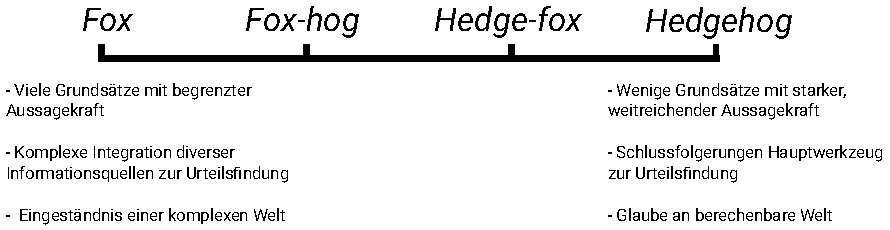
\includegraphics[scale=1]{Grafiken/Hedgehog_Fox.pdf} 
\label{pic:Hedgehog_Fox}
\end{figure}
\emph{Hedgehogs} haben einige wenige Glaubenssätze, die sie nutzen um
Erklärungen für die unterschiedlichsten Dinge abzuleiten (vgl. \cite{Tetlock},
S.~73). Sie bemühen sich, Fakten in Einklang mit ihren präferierten Grundsätzen
zu bringen und fällen ihre Urteile, indem sie Schlussfolgerungen aus einer
kleinen Menge an Überzeugungen ziehen. Zudem tendieren \emph{hedgehogs}
zu intellektuellem \glqq{Geiz}\grqq (\emph{parsimony}) (vgl.\cite{Tetlock}, 
S.~20). Dies bedeutet, dass sie nur ungerne neue Grundsätze
aufstellen und stattdessen versuchen, mit ihren wenigen, schon vorhandenen
Glaubenssätzen weitreichende Erklärungen für eine große Bandbreite an Phänomenen
zu erhalten. Zudem zeichnen sich \emph{hedgehogs} durch eine starke
Selbstsicherheit in Bezug auf die Genauigkeit ihrer Prognosen und Urteile aus
(vgl. \cite{Tetlock}, S.~73). \\ \\
\emph{Foxes} hingegen sind skeptisch bezüglich starker Glaubenssätze, die alles
umspannende Erklärungen liefern sollen. Stattdessen vertrauen sie auf viele
Grundsätze mit begrenzter Aussagekraft (\emph{tricks of their trade}) (vgl.
\cite{Tetlock}, S.~73). Weiterhin ist die Urteilsfindung bei \emph{foxes} keine
reine Übung in deduktiver Logik (vgl. \cite{Tetlock}, S.~73), sondern benötigt
die Integration diverser Informationsquellen. \emph{Foxes} sind eher zaghaft,
wenn es darum geht, ihre eigenen Fähigkeiten als Prognostiker zu loben (vgl.
\cite{Tetlock}, S.~73-74). \\ \\
\begin{figure}%[!hbt]
\centering
\caption{Leistungsunterschiede bei den \emph{forecasting exercises} in
  Abhängigkeit vom \emph{cognitive style} der Teilnehmer}
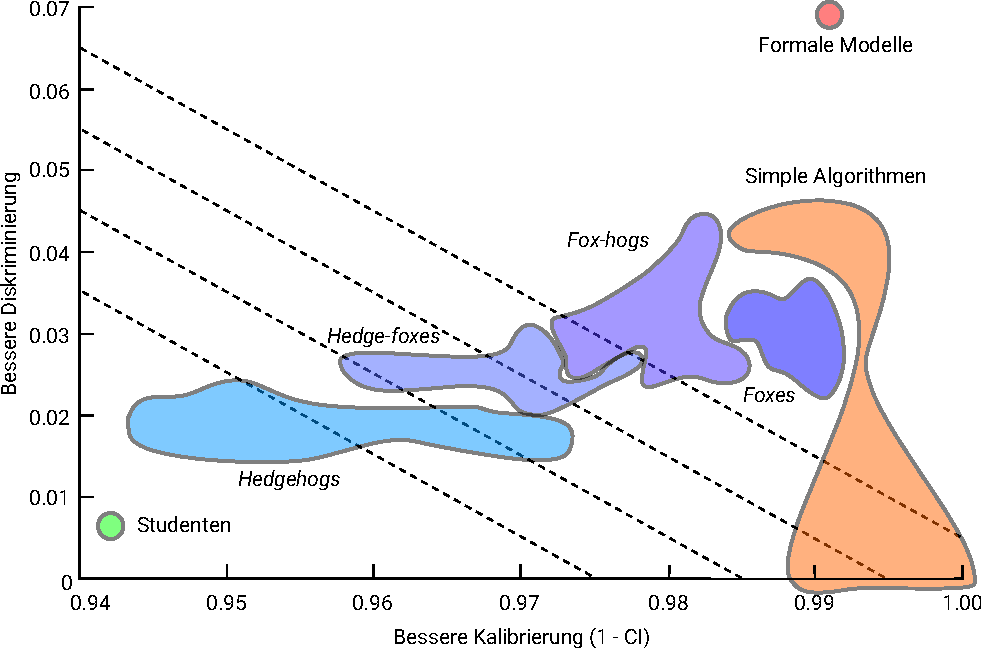
\includegraphics[scale=0.88]{Grafiken/Tetlock_2_Ink.pdf} 
\label{pic:Tetlock_2}
\end{figure}
Ein Ergebnis von Tetlocks \emph{forecasting exercises} wurde bereits in
Abbildung~\ref{pic:Tetlock_1} aus Teil~\ref{part:Schw_Vorhersagen} erläutert.
Dort war ersichtlich, dass die Experten im Vergleich zu statistischen
Algorithmen schlecht abschnitten. Abbildung~\ref{pic:Tetlock_2} zeigt nun ein
differenzierteres Bild von der Leistung der Experten.  
% Urteilskraft einzelner Experten bezüglich Kalibrierung und Diskriminierung
% variiert 
%\subsection{Analyse der Ergebnisse der Forecasting Exercises}

% (vgl. \cite{Tetlock}, S.~XXX)

% parsimony lohnt nicht (S. 68)
Tetlock ist der Meinung, dass die Kernaufgabe politischer Weltanschauungen
nicht die Erstellung möglichst korrekter Prognosen ist, sondern die
Aufrechterhaltung einer bequemen Illusion von Berechenbarkeit
(vgl. \cite{Tetlock}, S.~39). Somit sind die Ergebnisse schlecht, weil
nüchterner Realismus unerwünscht ist. Die Aufrechterhaltung von Glaubenssätzen,
die zum kollektiven Zusammenhalt beitragen, hat höhere Priorität.

Insgesamt wird die Befürchtung, dass sich Menschen durch Wunschdenken leiten
lassen (vgl. \cite{Eisenfuehr}, S.~181) und dass sie das oft tun, von Tetlocks
Arbeit bestätigt.


\begin{table}
\centering
\caption{Ausgewählte Beispiele für kognitive Verzerrungen}
\label{tab:Kognitive_Verzerrungen}
\scalebox{0.7}{
\begin{tabular}{ |l|l|l|  }
\hline
\textbf{Bezeichnung der kognitiven Verzerrung} & \textbf{Sinngemäße Übersetzung}
  & \textbf{Kurzbeschreibung} \\
\hline
{ \large \emph{Anchoring} } & Ankereffekt
  & Beharren auf einer ersten \\
& & Schätzung eines Wertes; \\
& & unzureichende Anpassung\\
& & nach weiterem Überlegen.\\
\hline
{ \large \emph{Attribution bias} } & Zuschreibungsfehler
  & Die Tendenz, Erfolge \\
& & seinen eigenen Fähigkeiten \\
& & zuzuschreiben; \\
& & Misserfolge hingegen \\
& & externen Zuständen. \\
\hline
{ \large \emph{Availability bias} } & Verfügbarkeitsfehler
  & Beispiele für Szenarien, \\
& & die unmittelbar mit einem \\
& & Ereignis assoziiert werden, \\
& & bestimmen die Einschätzung \\
& & dieses Ereignisses. \\
\hline
{ \large \emph{Base rate neglect} } & Vernachlässigung von Basisraten
  & Vernachlässigung allgemeiner \\
& & Wahrscheinlichkeiten und \\
& & Konzentration auf fallspezifische \\
& & Informationen. \\
\hline
{ \large \emph{Cognitive conservatism} } & Kognitiver Konservatismus
  & Weigerung von Menschen, \\
& & Fehler zuzugeben und \\
& & ihre Meinung zu ändern. \\
\hline
{ \large \emph{Gambler's fallacy} } & Irrtum des Glücksspielers
  & Der irrtümliche Glaube an \\
& & regelmäßige Muster \\ 
& & in zufälligen Prozessen. \\
\hline
{ \large \emph{Hindsight bias} } & Rückschaufehler
  & Der Versuch eine Einschätzung \\
& & eines Ereignisses, nach dessen \\
& & Eintreten, rückwirkend zu \\
& & verändern. \\
\hline
{ \large \emph{Overconfidence effect} } & Selbstüberschätzung
  & Überschätzung der Richtigkeit \\
& & eigener Urteile. \\
\hline
\end{tabular}
}
\end{table}

\subsection{Auswirkungen von Tetlocks Forschungsergebnissen}

\section{Bestandteile von \emph{predictive analytics}}

Bei \emph{predictive analytics} werden Daten mit Hilfe von geeigneten Methoden
verarbeitet, um verschiedene Arten von Prognosen zu ermöglichen. Dem
Datenanalysten stehen für diese Aufgabe Computeranwendungen zur Verfügung.
Diese Programme lesen die Daten ein, führen die notwendigen Berechnungen aus und
ermöglichen eine graphische Aufbereitung der Ergebnisse. \\ \\
Standardisierte
Vorgehensmodelle können helfen, die Arbeitsschritte einer Datenanalyse zu
vereinheitlichen. Ein Beispiel für ein solches Vorgehensmodell ist CRISP-DM \xcom.

\subsection{CRISP-DM Vorgehensmodell}

\subsection{Daten}

\subsubsection{Elementare Datentypen}

Bei Daten lassen sich verschiedene elementare Typen\footnote{Alternativ dazu
spricht man vom Skalenniveau (\emph{scale of measurement}) als eine
Eigenschaft von Daten und Variablen.} unterscheiden.
Je nach Datentyp einer
Variablen, werden ihre Werte unterschiedlich interpretiert. Zudem können
bestimmte mathematische Operationen nur mit Variablen eines bestimmten Typs
durchgeführt werden. Die Datentypen werden im folgenden Text genauer erläutert
(vgl. \cite{Arens}, S.~1229 und \cite{McCarthy}, S.~28-29).\\ \\
Der \glqq{einfachste}\grqq Datentyp ist eine nominal skalierte Variable. 
Werte von nominal skalierten Variablen werden als Namen
interpretiert. Weiterhin ist es nicht sinnvoll diese Art von Variablen zu
ordnen. Es lässt sich lediglich feststellen, ob zwei Variablen
gleich oder ungleich sind. Ein Beispiel für eine nominal skalierte Variable ist
der Name einer Stadt. Die Werte sind dann konkrete Städtenamen wie
\glqq{München}\grqq oder \glqq{Berlin}\grqq. Als Operationen stehen nur $=$
oder $\neq$ zur Verfügung, weil Aussagen wie 
\glqq{München}\grqq$=$\glqq{München}\grqq oder
\glqq{München}\grqq$\neq$\glqq{Berlin}\grqq sinnvoll sind. Nicht sinnvoll wären
dagegen Vergleiche wie \glqq{München}\grqq$<$\glqq{Berlin}\grqq
\footnote{Der Vergleich wäre sinnvoll, wenn mit der Nennung des Namens 
z. B. implizit die Größe der Stadt gemeint wäre. Dies ist hier aber nicht der
Fall.}.
Weitere Beispiele für nominal skalierte Variablen sind Geschlecht, Augenfarbe
oder Postleitzahl. \\ \\
Etwas mehr Möglichkeiten stehen zur Verfügung, wenn eine ordinal skalierte
Variable vorliegt. Für eine solche Variable ist eine Ordnung sinnvoll, sodass
alle Vergleichsoperationen möglich sind. Eine Kleidungsgröße (\texttt{S},
\texttt{M}, \texttt{L}) ist ein Beispiel für eine ordinal skalierte
Variable. Im Gegensatz zum Beispiel mit den Städtenamen ist ein Vergleich wie
\texttt{S} $<$ \texttt{M} hier sinnvoll. \\ \\
Wird eine Variable auf einer Intervallskala definiert, sind ihre Werte
numerisch.
Zusätzlich zu
allen Operationen von nominal und ordinal skalierten Variablen können hier auch
Additionen und Subtraktionen ausgeführt werden. Ein Beispiel hierfür sind
Temperaturen in °C, die addiert und subtrahiert werden können. Allerdings sind
20~°C nicht das Doppelte von 10~°C. Hier kann man erkennen, dass es bei
Intervallskalen nicht sinnvoll ist, Verhältnisse zu berechnen. Der Grund
hierfür ist, dass der Nullpunkt einer Intervallskala nicht mit dem absoluten
Nullpunkt einer Größe identisch sein muss. So sind 0~°C nicht der absolute
Nullpunkt für die Temperatur. Wenn man sinnvolle Verhältnisse berechnen will,
wird eine Proportionalskala benötigt. \\ \\
Eine auf einer Proportionalskala definierte Variable hat numerische Werte, für
die alle zuvor erwähnten mathematischen Operationen definiert sind und
zusätzlich auch Multiplikation und Division möglich sind.
%Insbesondere ist es sinnvoll Verhältnisse zu berechnen.
So führt eine
Multiplikation einer Länge in Metern mit der Konstante 2 zu der doppelten Länge.
Ist das Verhältnis zweier Längen gleich 10, so ist die eine Länge 10
mal so groß wie die andere. Weiterhin führt die Multiplikation zweier Längen
in m zu einer korrekten Fläche in $\textrm{m}^2$. Die Ergebnisse wären nicht
korrekt, wenn der Nullpunkt der Meterskala nicht mit dem Nullpunkt der
Längenskala identisch wäre, wie es bei Intervallskalen der Fall ist. \\ \\
Nominal und ordinal skalierte Variablen sind qualitative Variablen.
Variablen, die auf Intervall- oder Proportionalskalen definiert sind, werden
hingegen als quantitative oder kardinale Variablen bezeichnet.
Weiterhin werden qualitative Variablen auch als kategorisch
(\emph{categorical}) bezeichnet, quantitative als numerisch (\emph{numeric})
und je nach Wertebereich als diskret (\emph{discrete}, ganzzahlige Werte) oder
kontinuierlich (\emph{continuous}, Fließkommawerte). \\ \\
Tabelle~\ref{tab:Skalen} zeigt eine Zusammenfassung der verschiedenen Datentypen
und der erlaubten Operationen\footnote{
Basierend auf Tabelle 2.2 in \cite{Runkler}, S.~8}.
\begin{table}
%\footnotesize
\centering
\caption{Übersicht der Datenskalen}
\label{tab:Skalen}
\scalebox{0.7}{
\begin{tabular}{ |l|l|l|l|  }
\hline
\textbf{Skala} & \textbf{Sinnvolle Operationen}
  & \textbf{Beispielgrößen} & \textbf{Beispielwerte} \\
\hline
Nominal & Gleichheit ($=, \neq$) & Name, & \glqq{Julia}\grqq,
  \glqq{Klaus}\grqq \\
& & Geschlecht & \texttt{M}, \texttt{W} \\
\hline
Ordinal & Gleichheit ($=, \neq$), & Kleidungsgröße & \texttt{S}, \texttt{M},
  \texttt{L} \\
        & Vergleiche ($<, >, \ldots$) & & \\
\hline
Intervall & Gleichheit ($=, \neq$), & Jahresangabe, & 2015~n.Chr. \\
  & Vergleiche ($<, >, \ldots$), & Temperatur in Grad Celsius & 20~°C \\
  & Addition ($+$), Subtraktion ($-$), &  &  \\
\hline
Proportional & Gleichheit ($=, \neq$), & Alter, & 21 Jahre \\
  & Vergleiche ($<, >, \ldots$), & Temperatur in Kelvin & 273.4~K \\
  & Addition ($+$), Subtraktion ($-$), &  &  \\
  & Multiplikation ($\cdot$), Division ($/$) & & \\
\hline
\end{tabular}
}
\end{table}


\subsubsection{Information Management (Data Warehouse)}

\subsubsection{Datenabhängige Ziele}

\paragraph{\ldots}

\paragraph{Beschreibung der Daten}

\paragraph{Klassifikation}

\paragraph{Zeitreihenanalyse}

\subsection{Methoden}

\begin{figure}%[!hbt]
\centering
\caption{\emph{Predictive analytics} Methoden aus der Anwenderperspektive.}
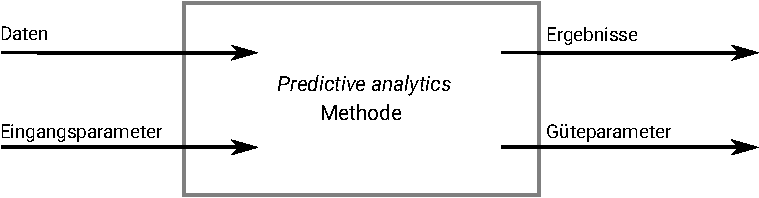
\includegraphics[scale=1.0]{Grafiken/PA_Methoden_Ink.pdf} 
\label{pic:PA_Methoden}
\end{figure}

\subsubsection{Die Großen Drei}

\paragraph{Regression}

\paragraph{Entscheidungsbäume}

\paragraph{Neuronale Netze}

\subsubsection{Zeitreihenanalyse}

\subsubsection{\ldots}

\subsection{Werkzeuge}

\subsection{(Kreative) Freiheitsgrade bei der Implementierung eines
  Vorhersagemodells}

\section{Anwendungsbeispiele}

\subsection{Allgemeine Anwendungsfelder (siehe SAP Artikel)}

\subsection{\ldots}

\section{Allgemeine Risiken bei der Nutzung von Predictive Analytics}

Es existieren Risiken, die dazu führen können, dass die Ziele einer
Datenanalyse nicht oder nicht in vollem Umfang erreicht werden können.
Im folgenden Text werden einige dieser Risiken erläutert.

\subsection{Risiko der Unverhältnismäßigkeit}

Die Anwendung von Predictive Analytics ist mit einem hohen Aufwand verbunden.
Dabei spielen die Kosten für die Datenerhebung eine wesentliche Rolle.
Zusätzlich werden für die Datenanalyse Kenntnisse aus verschiedenen
Fachrichtungen benötigt. So sind einerseits anwendungsspezifische Kenntnisse
zur Interpretation der Daten und der Ergebnisse wünschenswert. Andererseits
werden zur Durchführung der Datenanalyse Kenntnisse in Mathematik, Statistik und
Informatik benötigt. \\ \\
Aus diesem Grund besteht das Risiko, dass die Kosten einer Anwendung von
Predictive Analytics den Nutzen übersteigen. Es ist auch möglich, dass das
gleiche Ergebnis mit einer einfacheren, kostengünstigeren Methode erreicht
werden kann. In diesem Fall würde die Anwendung eines aufwändigen Predictive
Analytics Verfahrens wertvolle Ressourcen binden, die an anderer Stelle stärker
gebraucht werden. \\ \\
Somit ist es wichtig, Betrachtungen zu Alternativkosten \todo{gls eintrag}
in die Planung von \emph{predictive analytics} Anwendungen einzubeziehen. 

\subsection{Risiken bei der Datenerhebung}

Trainingsdaten spiegeln nicht (mehr) das Verhalten des Systems wider.

\subsubsection{\ldots}

\subsection{Risiken bei der Interpretation der Daten}

\subsection{Risiken bei der Interpretation der Ergebnisse}

Wenn die Ergebnisse der Datenanalyse zur Entscheidungsunterstützung herangezogen
werden, beeinflussen sie das Verhalten der Entscheidungsträger. Dies kann zur
Entstehung problematischer psychosozialer Effekte führen. Zwei Beispiele hierfür
werden nun erläutert.

\subsubsection{Prognose verändert das Verhalten des Systems }

Die Ergebnisse von Vorhersagen werden von Menschen interpretiert,
die daraufhin ihr Verhalten anpassen. Dies kann zu Rückkopplungseffekten führen,
die von negativen Auswirkungen im Sinne einer
\glqq{Selffulfilling} Prophecy\grqq begleitet werden können
(vgl. \cite{Crossman}). Bestimmte Prognosen können beispielsweise von einer 
Interessengruppe als Bestätigung ihrer Agenda interpretiert werden, wobei
anders lautende Vorhersagen ignoriert werden. Dadurch bestärkt, setzt die Gruppe
ihre gewünschten Handlungsoptionen um. Dies ruft den vorhergesagten Effekt
jedoch erst hervor.

\subsubsection{Ignorieren der Unsicherheiten bei der Prognose}

Es besteht die Gefahr, dass die Unsicherheiten von Vorhersagen ignoriert werden
und die Prognose als eine Gewissheit betrachtet wird. Somit wird möglichen,
alternativen Entwicklungen bei der Entscheidungsfindung nicht genügend Bedeutung
beigemessen. Dies kann dazu führen, dass Risiken falsch kalkuliert werden und
in der Zukunft nicht genügend Handlungsoptionen zur Verfügung stehen.


\chapter{Predictive Analytics im öffentlichen Sektor}

\begin{figure}%[!hbt]
\centering
\caption{Risikomatrix für die Nutzung maschineller Entscheidungshilfen.}
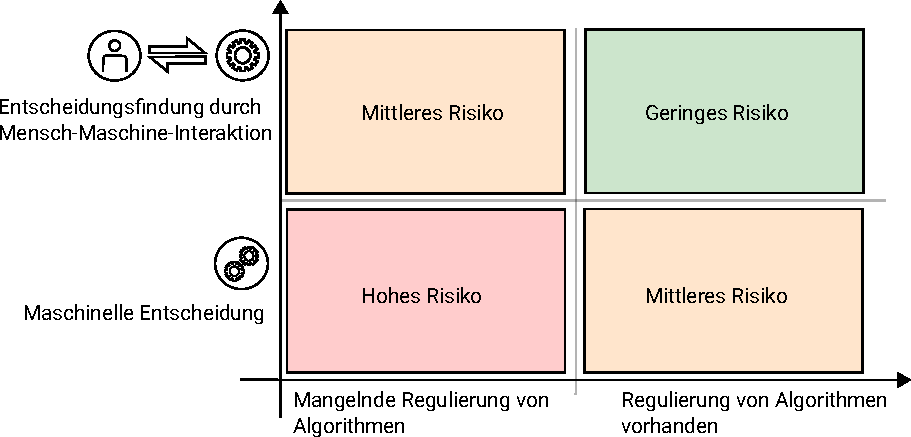
\includegraphics[scale=1.0]{Grafiken/Risk_Matrix_Ink.pdf} 
\label{pic:Risiko_Matrix}
\end{figure}

\section{Übersicht}

\section{Thematische Schwerpunkte}
\todo{Wo könnte der größte Nutzen liegen?}

\todo{vorläufig:}

\subsection{Öffentliche Verwaltung}

\subsubsection{Daten in der öffentlichen Verwaltung}

\paragraph{Open Data Portale ( GovData.de )}

\subsubsection{Organisationseinheiten für Predictive Analytics}

\paragraph{\ldots}

\subsection{Gesundheit}

\subsection{Bildung}

\chapter{Gegenwärtige Anwendungen}

\section{Predictive Analytics in Finanzbehörden}

\section{Google Flu Trends}

\section{Predictive Policing}

\section{Cambridge Analytica}

% TODO Auflistungstabelle
% Kategorie | Anwendung | Beispiel

\chapter{Zukunftsperspektiven}

\section{\ldots}

\section{Einschätzung der politischen Stimmungslage}

\section{Vorhersage kultureller Unterschiede}

\chapter{Zusammenfassung und Fazit}

%%%%%%%%%%%%%%%%%%%%%%%%%%%%%%%%%%%%%%%%%%%%%%%%%%%%%%%%%%%%%%%%%%%%%%%%%%%%%%%%
\appendix
\chapter{Probablility Scoring - Vertiefung}

\chapter{Predictive Analytics mit R}

\section{Tabellenkalkulationen versus R}

Inhalt vom ersten Anhang.

\section{Beispielhafte Auswertung eines Datensatzes}

Inhalt des zweiten Anhang.

%%%%%%%%%%%%%%%%%%%%%%%%%%%%%%%%%%%%%%%%%%%%%%%%%%%%%%%%%%%%%%%%%%%%%%%%%%%%%%%%
\bibliography{Bibliographie/Bibli.bib}{}
\bibliographystyle{babplain}

\listoffigures
\listoftables
\printglossary[title=Glossar]
\printglossary[type=\acronymtype, title=Akronyme]
% keine deutschen Überschriften
%\printglossaries 

\end{document}


